\documentclass[master=cws, twoside]{kulemt} \setup{title={Programmeren en
  Bewijzen met Dependently Typed Talen}, author={Toon Nolten}, promotor={Dr.\
  Dominique Devriese \and Prof.\,dr.\,ir.\ Frank Piessens},
  assessor={Prof.\,dr.\ Marc Denecker \and Dr.\ Thomas Heyman},
assistant={Jesper Cockx}}
% De volgende \setup mag verwijderd worden als geen fiche gewenst is.
\setup{filingcard, translatedtitle={Programming and Proofs in Dependently Typed
  Languages}, udc=681.3, shortabstract={In this thesis we present two case
    studies, both in Agda, a fully dependently typed programming language, and
    in Haskell, a functional programming language with a Hindley-Milner style
    type system. After formulating a model of a problem in Agda, we mimic this
    model in Haskell, relying on Glasgow Haskell Compiler extensions to provide
    type system features we lack in standard Haskell. We try to illustrate how
    much, or little effort goes into static verification. And hint at reducing
    reliance on test suites by encoding simple properties in our types.}}

% TODO: toggle voor gedrukte versie?
\usepackage[pdfusetitle,colorlinks,linkcolor=black,citecolor=black,urlcolor=black,plainpages=false]{hyperref}

\usepackage{amsmath}
\usepackage{amssymb}
\usepackage[outputdir=_build]{minted}
\usepackage{underscore}
\usepackage{subcaption}
\usepackage{import}
\usepackage{textgreek}

% Missing unicode characters for Agda
\usepackage{MnSymbol}
\DeclareUnicodeCharacter{"2237}{$\squaredots$}
\DeclareUnicodeCharacter{"25C2}{$\blacktriangleleft$}
\DeclareUnicodeCharacter{"25B8}{$\blacktriangleright$}
\DeclareUnicodeCharacter{"1D9C}{$^{c}$}
\DeclareUnicodeCharacter{"225F}{$\stackrel{?}{=}$}
\DeclareUnicodeCharacter{"25A0}{$\blacksquare$}

% More readable minted commands
\newmintinline[iagda]{agda}{}
\newmintinline[ihask]{haskell}{}

\newmintedfile[inputagda]{agda}{}
\newmintedfile[inputhaskell]{haskell}{}

\begin{document}

\begin{preface} Ik heb dit thesisonderwerp gekozen omdat ik erg geïnteresseerd
  ben in programmeertalen. Van jongs af aan heb ik me altijd afgevraagd hoe
  dingen werken. Eén van de grootste raadsels was hoe een computer nu eigenlijk
  werkt. Ik heb redelijk snel geleerd dat een computer eigenlijk niets meer is
  dan een machine die een stroom van bits omzet in een andere stroom van bits.
  Niet dat ik daarmee volledig begreep hoe een computer werkt op het niveau van
  bits en bytes, maar ik kon me er toch iets bij voorstellen. Waar bij mij het
  interessantste probleem zat was de omzetting van een programma zoals wij het
  zouden schrijven naar zo een stroom van bits. Stilaan heb ik dan geleerd wat
  een compiler is en dat bracht eigenlijk alleen meer problemen met zich mee:
  ``Hoe kan de C compiler in C geschreven zijn?'' Dit maar om aan te geven dat
  ik het een fascinerend onderwerp vind. De interesse in dependent types is
  eigenlijk eerder toevallig gekomen. Ik had de beschrijving van het onderwerp
  al eens gelezen en daarbij moest ik meteen denken aan hoe het typesysteem van
  Java mij al had tegengewerkt in vorige opdrachten. Maar ik dacht tegelijk ook
  aan Haskell wat een veel aangenamer typesysteem heeft. En die dissonantie is
  eigenlijk de reden dat ik voor dit onderwerp gekozen heb. Waarom is het ene
  typesysteem eerder aangenaam om mee te werken en het andere niet? En
  belangrijker nog: ``Hoe ver kan een typesysteem gaan?''

  Ik wil ook nog een aantal mensen bedanken. In de eerste plaats mijn
  begeleider Jesper en mijn promotor Dominique, zij hebben mij tegelijk op het
  juiste pad gezet en mij veel zelfstandigheid gegeven in wat ik juist wou doen
  en hoe ik het wou doen. Ook heb ik veel gehad aan discussies in de \#agda en
  \#haskell IRC kanalen op het freenode netwerk waarbij ik vermijd namen te
  noemen omdat de kans groot is dat ik iemand vergeet. Verder wil ik mijn vader
  bedanken die altijd bereid was te luisteren naar een al te vaak ingewikkelde
  uitleg wanneer ik me een nieuw concept probeerde eigen te maken. Natuurlijk
  kan ik niet vergeten mijn moeder te bedanken voor het rusteloze aandringen om
  nu toch eindelijk is aan die thesis te beginnen werken. Tenslotte wil ik mijn
  grootvaders bedanken die me met hun uitgebreide kennis geïnspireerd hebben om
  altijd vragen te blijven stellen.
\end{preface}

\tableofcontents*

\begin{abstract}
  Dependent types vormen een krachtig middel om bepaalde eigenschappen te
  coderen in het typesysteem. Op deze manier moeten we niet telkens aan alle
  eigenschappen proberen denken. Wat de computer voor ons kan doen, moeten we
  zelf niet doen. In programmeertalen is er al lang een tendens om meer door de
  computer zelf te laten doen, bijvoorbeeld het geheugenbeheer met garbage
  collectors. Wat typesystemen betreft is dit jammer genoeg nog niet het geval.
  Er wordt wel onderzoek verricht maar dit komt zelden terecht in een van de
  talen die voor alledaagse taken worden gebruikt. Haskell is één van de
  uitzonderingen op deze regel. Het is een taal die zijn nut in de praktijk al
  bewezen heeft. En die tegelijkertijd nog het onderwerp is van onderzoek om
  betere technieken te vinden voor onder andere typesystemen en concurrency.
  Agda staat in vergelijking nog in de kinderschoenen maar dit maakt het ook
  mogelijk om op een sneller tempo te experimenteren.

  In deze thesis proberen we aan de hand van twee gevalstudies een beter zicht
  te krijgen op programmeren met dependent types. Waarvoor het nuttig kan zijn:
  meer concepten uitdrukken op een type safe manier en statisch eigenschappen
  verifiëren bijvoorbeeld. Wat er aan schort: geen inferentie van types,
  \emph{verbose}. En hoe een taal die eigenlijk geen dependent types heeft zich
  verhoudt tot een dependently typed taal.
\end{abstract}

\mainmatter

\chapter{Inleiding}
\label{inleiding}

%%%%%%%%%%%%%%%%%%%%
% Chapters

\chapter{Programmeertalen}
\label{ch:agda-haskell}


\section{Inleiding}

In dit hoofdstuk beschrijven we de programmeertalen die gebruikt zijn in de
gevalstudies. Er moet ergens een grens getrokken worden die bepaald wat wel en
niet uitgelegd wordt, deze thesis veronderstelt dat de lezer vertrouwd is met
getypeerd functioneel programmeren. Omdat Agda minder bekend is, is de uitleg
hierover uitgebreider dan die over Haskell. Het enige dat we voor Haskell
moeten uitleggen zijn namelijk de extensies van GHC \ref{ghc} die we gebruiken.
Merk op dat overal waar code getoond wordt, het symbool
{\tiny\ensuremath{\hookrightarrow}} gebruikt wordt om aan te duiden dat een
regel die te lang was op die regel verder gaat, dit resulteert niet altijd in
geldige code dus bij het overnemen moet hierop gelet worden.


\section{Agda}

Agda is een dependently typed programmeertaal. Talen met dependent types zijn
dankzij de Curry-Howard correspondence ook bruikbaar als bewijsassistent. In
vele andere talen met dependent types ligt de nadruk ook eerder op het gebruik
als bewijsassistent dan wel als programmeertaal.

\subsection{Dependent Types}

Het belangrijkste verschil tussen Agda en andere functionele programmeertalen
is het typesysteem. Een dependent type is een type dat afhangt van een waarde.
De voorgaande zin legt eigenlijk alles uit dat belangrijk is aan dependent
types maar iemand die nog niet vertrouwd is met dependent types zal hier weinig
van opsteken. Vandaar overlopen we een aantal voorbeelden in Agda: eerst om de
syntax te verduidelijken, daarna om te illustreren wat dependent types nu
eigenlijk zijn.

De definitie van nieuwe types gebeurt gelijkaardig als in andere getypeerde
functionele programmeertalen. Een \iagda{data} sleutelwoord wordt gevolgd door
de naam van het type, een dubbel punt, het type van het type, dan het
sleutelwoord \iagda{where} en op de volgende regels de constructors met hun
type. Nemen we als voorbeeld een definitie voor natuurlijke getallen:

%----------------------------------------%
\begin{minted}[fontsize=\small]{agda}
  data Nat : Set where
    zero : Nat
    suc  : Nat → Nat
\end{minted}

Dit geeft ons een unaire voorstelling van de natuurlijke getallen, het getal 2
stellen we bijvoorbeeld voor als volgt: \iagda{suc (suc zero)}. Een verschil
met andere talen is dat we het type van het type moeten opgeven.  In
dependently typed talen is de scheiding tussen types en waarden fundamenteel
opgeheven. Het type van de meeste eenvoudige types is in Agda \iagda{Set}, wat
eigenlijk \iagda{Set₀} is. Het type van \iagda{Set₀} is \iagda{Set₁} en deze
hiërarchie gaat in theorie oneindig ver door. Haskell heeft gelijkaardige
concepten maar daar gaat de hiërarchie niet erg ver door. De hiërarchie gaat
als volgt in Haskell, met de Engelse termen omdat ze niet allemaal een goede
vertaling hebben: een value heeft een type, een type heeft een kind, een kind
heeft een sort en hier stopt de hiërarchie. Het dichtste equivalent van
\iagda{Set} is in Haskell het kind \ihask{*}, \ihask{*} heeft nog sort
\ihask{BOX} maar \ihask{BOX} heeft zelf sort \ihask{BOX}. Merk op dat
\ihask{BOX} enkel en alleen een intellectueel concept is, het is niet uit te
drukken in Haskell zelf.  Het tweede verschil met een type declaratie in een
taal zoals Haskell is dat we het type van elke constructor moeten opgeven, voor
\iagda{Nat} is dit heel eenvoudig. In het volgende voorbeeld wordt duidelijker
waarom we deze types moeten specificeren.

Dit voorbeeld wordt vaak gebruikt om het concept van dependent types te
illustreren. Deze code komt uit de Agda Standard Library \ref{agda:stdlib} maar
is licht aangepast om het voorbeeld eenvoudiger te maken.

%----------------------------------------%
\begin{minted}[fontsize=\small]{agda}
  data Vec (A : Set) : ℕ → Set where
    []  : Vec A zero
    _∷_ : ∀ {n} (x : A) (xs : Vec A n) → Vec A (suc n)

  head : ∀ {n} {A : Set} → Vec A (suc n) → A
  head (x ∷ xs) = x
\end{minted}

\iagda{Vec} is het type voor lijsten met een vaste lengte, vanaf nu noemen we
dit vectors. Hier zien we twee nieuwe dingen, het type \iagda{Vec} verwacht nog
twee argumenten. Het eerste is de parameter voor de dubbel punt, \iagda{A} met
als type \iagda{Set} dus \iagda{A} is een eenvoudig type. Het tweede is de
index van het type \iagda{ℕ}, dit is de naam van het type voor natuurlijke
getallen uit de standard library, het verschil tussen een index en een
parameter is dat een index voor elke constructor kan variëren terwijl een
parameter voor alle constructors hetzelfde is. Een type met indices noemen we
ook wel een inductive family \ref{indfam}. De lege vector, \iagda{[]}, heeft
lengte nul, het type is \iagda{Vec A zero}: het is dus een vector van elementen
van type \iagda{A} met lengte \iagda{zero}. De constructor die langere vectoren
maakt, verwacht een element, \iagda{x} van type \iagda{A}, een vector met
elementen van hetzelfde type \iagda{A} en een bepaalde lengte \iagda{n},
namelijk \iagda{xs} met als type \iagda{Vec A n}, en geeft een vector terug
waarvan de lengte één groter is, \iagda{Vec A (suc n)}. De \iagda{head}
functie, die het eerste element van een vector terug geeft kan dan eisen dat ze
enkel werkt op vectoren met een lengte groter dan nul, vectoren met type
\iagda{Vec A (suc n)}. Als de lengte niet in het type opgenomen is, kan een
functie er ook geen voorwaarden aan opleggen. Zo moet de \ihask{head} functie
voor gewone lijsten in Haskell een fout opwerpen wanneer ze opgeroepen wordt
met een lege lijst als argument.  Dit is een heel eenvoudig voorbeeld en
hieruit blijkt niet welke van de twee een betere manier is om lijsten voor te
stellen.  Het laat wel zien wat het betekent voor een type om af te hangen van
een waarde. Wat we ook zien, zowel in het type van \iagda{_∷_} als \iagda{head}
is \iagda{∀ {n}}, de universele kwantor zorgt dat \iagda{n} eender wat kan zijn
zolang het voldoet aan de eisen in de rest van het type. De accolades rond
\iagda{n} en in het type van \iagda{head} ook rond het type van het volgende
argument, \iagda{{A : Set}}, duidt aan dat deze argumenten impliciet zijn, ze
worden afgeleid uit de context, in dit geval bijvoorbeeld uit het type van het
vector argument. Er is nog een ander soort impliciete argumenten in Agda,
instance arguments, deze worden aangeduid met dubbele accolades en worden op
een andere manier ingevuld, de typechecker zoekt naar een concrete instance in
de context, als er verschillende mogelijkheden zijn leidt dat tot een typefout.
Oorspronkelijk zijn instance arguments toegevoegd aan Agda als een eenvoudig
alternatief voor typeclasses uit Haskell.

Een meer uitgebreid voorbeeld uit een artikel dat het nut van dependent types
goed uitlegt \ref{TPoP}, laat zien dat dependent types zeer expressief zijn.
Het type \iagda{RA} laat toe om een relationele algebra expressie op te stellen
die correct is door constructie. Het artikel beargumenteert dat het in Haskell
niet mogelijk is om een interface naar een database te voorzien die evenveel
statische garanties biedt en even volledig - joins zijn zonder dependent types
moeilijk te typeren - is zonder gebruik te maken van preprocessing of
experimentele features. Dit betekent niet dat er geen libraries bestaan voor
Haskell die bepaalde eigenschappen statisch of dynamisch op leggen, maar wel
dat die beperkter zijn en minder statisch kunnen zijn. Statische correctheid is
handiger omdat ze geen uitvoerige testen noodzakelijk maakt.

%----------------------------------------%
\begin{minted}[fontsize=\small]{agda}
  data RA : Schema → Set where
    Read    : ∀ {s} → Handle s → RA s
    Union   : ∀ {s} → RA s → RA s → RA s
    Diff    : ∀ {s} → RA s → RA s → RA s
    Product : ∀ {s s'} → {_ : So (disjoint s s')} → RA s → RA s'
              → RA (append s s')
    Project : ∀ {s} → (s' : Schema) → {_ : So (sub s' s)} → RA s → RA s'
    Select  : ∀ {s} → Expr s BOOL → RA s → RA s
\end{minted}

Het type \iagda{Schema} stelt een schema van een relatie voor, door dit als
index op te nemen, kunnen we bepaalde eisen stellen aan de schema's waarop een
relationele expressie werkt. De \iagda{Read} constructor gelijkt een beetje op
een lege lijst omdat die aan de basis van elke relationele expressie moet
liggen, voor alle andere constructors voor een relationele expressie hebben we
al een relationele expressie nodig. \iagda{Read} bevat de informatie die
aangeeft in welke database de relatie te vinden is in een \iagda{Handle}. Zo'n
\iagda{Handle} heeft tevens een schema als index en kunnen we enkel opstellen
als de database inderdaad een relatie heeft die aan het schema voldoet. Voor de
unie van twee relaties, \iagda{Union}, en het verschil tussen twee relaties,
\iagda{Diff}, eisen we dat de schemas overeenkomen: een relatie kan maar een
unie zijn van twee relaties als alle attributen overeenkomen, eigenlijk moeten
de schema's niet hetzelfde zijn maar mogen ze permutaties van elkaar zijn maar
dit kan opgelost worden door de implementatie van \iagda{Schema}. De
constructor voor het cartesisch product, \iagda{Product}, heeft een impliciet
argument van het type \iagda{So (disjoint s s')}, de underscore duidt aan dat
we het argument niet gebruiken in de rest van het type maar moet er staan omdat
we een type van een impliciet argument niet zonder een variabele kunnen
opgeven. Het type \iagda{So (disjoint s s')} zorgt ervoor dat de schemas
\iagda{s} en \iagda{s'} disjunct zijn omdat een relatie geen twee attributen
met dezelfde naam kan hebben en een cartesisch product geen join is. Verder
zien we dat \iagda{Product} een relationele expressie opstelt waarvan het
resulterende schema de combinatie van de disjuncte schema's is. Voor de
projectie, \iagda{Project}, eisen we dat de attributen die we uit een relatie
willen projecteren inderdaad aanwezig zijn in de relatie. Het belangrijkste
kenmerk van de \iagda{Select} constructor kunnen we helaas niet uitleggen
zonder meer van het artikel over te nemen maar is niet belangrijk in de rest
van dit werk.

\subsection{Syntax}

Wat ook opmerkelijk is aan Agda, is de vrijheid die er is door de flexibele
syntax. Agda legt geen regels op in verband met hoofdletters voor types en
constructors en kleine letters voor functies, dit mes snijdt natuurlijk aan
twee kanten omdat types en functies minder gemakkelijk uit elkaar te houden
zijn. Wat waarschijnlijk de belangrijkste reden is om zulke regels niet af te
dwingen is dat er eigenlijk geen verschil is tussen waarden en types, een
functie is ook een waarde, het is dus ook niet logisch om artificieel een
verschil op te leggen in de schrijfwijze. Wat naamgeving betreft is nog een
belangrijk kenmerk dat alle unicode karakters toegelaten zijn. Hier wordt in de
standard library ook veel gebruik van gemaakt. Praktisch betekent dit dus dat
er goede ondersteuning moet zijn van de tekstverwerker en het lettertype waarin
je Agda code schrijft.

Een belangrijker kenmerk van de syntax in Agda is dat types, constructors en
functies gedefinieerd kunnen worden met mixfix notatie. Voor vectoren hebben we
al een infix constructor gezien, een tweede voorbeeld van zulke notatie is dit:

%----------------------------------------%
\begin{minted}[fontsize=\small]{agda}
  if_then_else_ : {A : Set} → Bool → A → A → A
  if true then x else y = x
  if false then x else y = y
\end{minted}

Deze functie kunnen we nu op twee manieren gebruiken. Met prefix notatie als we
de naam met underscores overnemen als volgt: \iagda{if_then_else_ true x y}. Of
zoals in de definitie in de mixfix vorm. Soms maakt dit de code gemakkelijker
leesbaar. Wat wel noodzakelijk wordt door zo'n flexibele notatie is het
veelvuldig gebruik van spaties, voor \iagda{if_then_else_} maakt dit weinig uit
want daar zijn de spaties logisch maar stel bijvoorbeeld dat dit een functie
is: \iagda{[_]}, dan moeten er spaties rond het argument, \iagda{[ x ]}, wat in
het begin vreemd aanvoelt maar nodig is omdat \iagda{[x]} een geldige naam zou
kunnen zijn voor een functie.

\subsection{Modules}

Agda heeft net als Haskell modules om code in te kunnen delen in verschillende
logische eenheden die eventueel over verschillende bestanden verdeeld kunnen
worden. In Agda kunnen we modules ook parametriseren, dit gaat in Haskell niet
maar is wel terug te vinden in bijvoorbeeld de ML \ref{ml} familie van talen.
Om een geparametriseerde module te gebruiken moeten we er waarden aan meegeven
overeenkomstig de types van de parameters. Op deze manier kunnen we er
bijvoorbeeld voor zorgen dat een module met sorteerfuncties enkel gebruikt
wordt voor elementen die een orderelatie hebben.

\subsection{Versie}

De gebruikte versies van Agda en de standard library in de rest van deze thesis
zijn respectievelijk \texttt{2.4.2.2} en \texttt{0.9}.


\section{Haskell}

Omdat we redelijk veel vergen van het typesysteem, komen we niet toe met
standaard Haskell zoals bijvoorbeeld geïmplementeerd in GHC maar hebben we een
aantal extensies nodig van GHC.

\subsection{Waarden op typeniveau}

Haskell heeft geen dependent types maar we hebben waarden nodig op het niveau
van types, in Haskell moeten we die dus voorstellen door types, en die types
moeten zelf een type hebben, wat in Haskell dus een kind is. Normaal kunnen we
in Haskell geen kinds definiëren maar me de extensie DataKinds gaat dit wel.
Deze extensie laat ons toe om zelf kinds te definiëren met bijhorende types
door onze gewone types te promoveren tot kinds en hun constructors te
promoveren tot types. Een voorbeeld maakt dit duidelijker:

%----------------------------------------%
\begin{minted}[fontsize=\small]{haskell}
  data Nat = Z | S Nat

  two :: Nat
  two = S (S Z)

  type_level_two :: S (S Z)
\end{minted}

We definiëren gewoon een type voor natuurlijke getallen en door de DataKinds
extensie wordt dit type een kind en de constructors types. Het kind \ihask{Nat}
is dus het kind van twee types namelijk \ihask{Z} en \ihask{S Nat}. De
\ihask{Nat} in \ihask{S Nat} is opnieuw het kind Nat niet het type. Omdat
dezelfde namen voor verschillende concepten af en toe verwarrend kunnen zijn en
het niet onmogelijk is dat we al een type \ihask{Z} gedefinieerd hadden, worden
types en constructors ook altijd gepromoveerd tot kinds en types die beginnen
met een apostrophe. Het type \ihask{Nat} wordt bijvoorbeeld altijd gepromoveerd
tot de kind \ihask{'Nat} en de constructor \ihask{Z} tot het type \ihask{'Z}.
Met deze extensie kunnen we dus waarden voorstellen op typeniveau waar de
extensie nog tekortschiet is dat de waarde \ihask{Z} en het type \ihask{Z}
volledig los van elkaar staan, buiten de naam. Er is ook geen waarde van het
type \ihask{Z}. In één van de volgende hoofdstukken gebruiken we een techniek
waarmee we de waarden op waardeniveau en typeniveau ongeveer kunnen verbinden.

\subsection{Inductive families}

In Haskell hebben we wel types die kunnen afhangen van andere types, een
voorbeeld hiervan is het \ihask{Maybe a} type en dit geeft ons de indices uit
Agda. Wat nog mist is de mogelijkheid om het type voor iedere constructor te
variëren. Met behulp van generalised algebraic data types uit de GADTs extensie
kunnen we dit wel. De KindSignatures extensie laat ons toe om bepaalde termen
te annoteren met een kind zoals we nu bepaalde termen een type annotatie kunnen
geven. Met deze twee extensies kunnen we eenvoudige inductive families
implementeren in Haskell, als voorbeeld beschouwen we het type voor vectors:

%----------------------------------------%
\begin{minted}[fontsize=\small]{haskell}
  data Vec :: * -> Nat -> * where
    V0 :: Vec a Z
    (:>) :: a -> Vec a n -> Vec a (S n)
\end{minted}

Het belangrijkste verschil met de definitie in Agda is dat het type van de
elementen nu niet hetzelfde zou moeten zijn voor elke constructor. Haskell laat
ons bijvoorbeeld toe te zeggen dat \ihask{V0} het type \ihask{Vec Int Z} heeft
en dat \ihask{(:>)} een vector met type \ihask{Vec Char (S n)} oplevert. We
moeten dus zelf beter opletten bij het definiëren van de types van de
constructors.

\subsection{Impliciete resolutie van een relatie}

Een relatie tussen twee types kunnen we voorstellen met een nieuw type, laten
we als voorbeeld de relatie tussen vlaggen en landen nemen:

%----------------------------------------%
\begin{minted}[fontsize=\small]{haskell}
  data Flag = DrieKleur | StarsAndStripes | UnionJack

  data Country = Belgium | USofA | UnitedKingdom

  data FlagCountry :: Flag -> Country -> * where
    Belg :: FlagCountry DrieKleur Belgium
    Amer :: FlagCountry StarsAndStripes USofA
    Engl :: FlagCountry UnionJack UnitedKingdom
\end{minted}

Als we nu in een type een vlag kennen en het land willen weten kunnen we dit
type gebruiken om dit te weten te komen: \ihask{flag -> FlagCountry flag
country -> country}, dit is eigenlijk niet geldig in Haskell maar het gaat om
het idee. Dit is soms te expliciet omdat we wel in het type van de relatie
geïnteresseerd zijn maar niet in de waarde zelf. In Haskell kunnen we
gebruikmaken van typeclasses om informatie impliciet te houden, de typeclasses
uit standaard Haskell laten maar een parameter toe. Omdat we voor een relatie
twee parameters nodig hebben, maken we gebruik van de MultiParamTypeClasses
extensie. De FlexibleInstances extensie laat ons toe om type variables te
gebruiken in de \ihask{instance} declaraties. De bijhorende typeclass voor het
vorige voorbeeld zou er als volgt uitzien:

%----------------------------------------%
\begin{minted}[fontsize=\small]{haskell}
  class FlgCntry (f :: Flag) (c :: Country)
  instance FlgCntry DrieKleur Belgium
  instance FlgCntry StarsAndStripes USofA
  instance FlgCntry UnionJack UnitedKingdom
\end{minted}

Het type van een functie die hiervan gebruik maakt, wordt niet minder expliciet
maar we moeten geen argument meer meegeven waar weinig informatie in zit:
\ihask{FlgCntry flag country => flag -> country}, dit is weer geen geldige
Haskell code maar het gaat om het idee.

\subsection{Versie}

De gebruikte versie van GHC in deze thesis is \texttt{7.6.3}.


\section{Besluit}

Met de kennis van de twee talen die we in dit hoofdstuk opgebouwd hebben,
kunnen we beginnen aan de gevalstudies. In de eerste gevalstudie bekijken we
een formalisering van de paden die een spelfiguur aflegt om zo fouten te kunnen
voorkomen. In de tweede gevalstudie implementeren we een soort zoekbomen,
red-black trees, met statische verificatie van de invarianten.

\chapter{Case: Verified Koopa Troopa Movement}
\label{ch:case-koopa}


\section{Inleiding}

Deze eerste gevalstudie is geïnspireerd door de populaire Mario \ref{mario}
franchise van Nintendo \ref{nintendo}, in het bijzonder Super Mario Bros.
\ref{supmario}. Er zijn verschillende vijanden in het spel maar hier beperken
we ons tot de schildpadachtige Koopa Troopas. Zoals wel vaker voorkomt bevatten
vele van de Mariospellen zogenaamde \emph{glitches}, fouten die uitgebuit
kunnen worden om bepaalde acties uit te voeren die normaal moeilijk of
onmogelijk zijn. Zo is er bijvoorbeeld een fout met een Koopa Troopa waardoor
Mario aan het einde van het level over de vlag kan springen, dit is normaal
niet mogelijk. De precieze fout is moeilijk uit te leggen maar ze is mogelijk
omdat een Koopa Troopa als het ware onder het level kan rondlopen, dit is in
figuur \ref{koopaglitch} te zien. Deze fout is eigenlijk de precieze inspiratie
van deze gevalstudie.

\begin{figure}
  \centering
  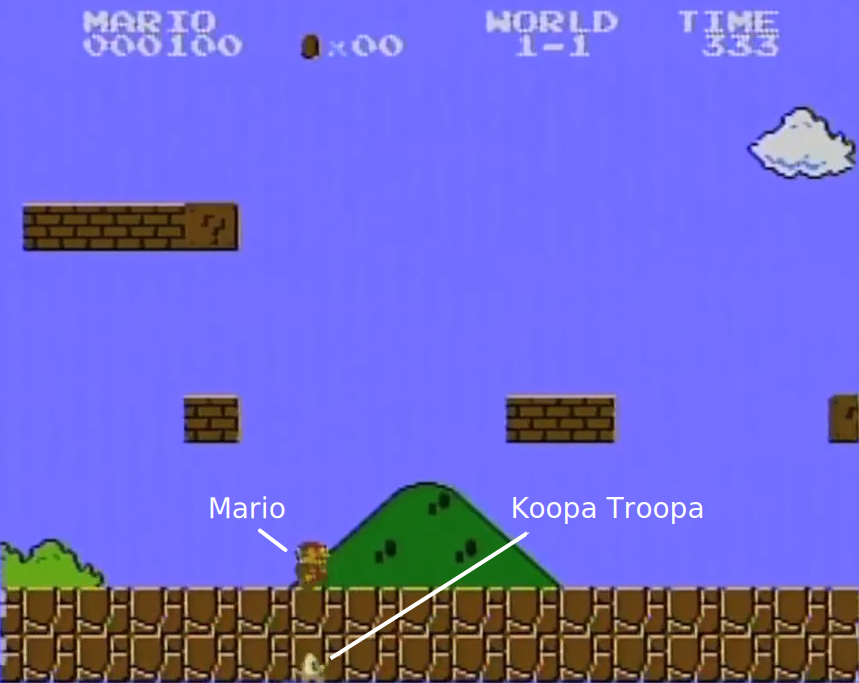
\includegraphics[width=\linewidth]{figures/KoopaTroopaGlitch}
  \caption{Onder Mario is nog net het hoofd van een Koopa Troopa te zien
           \ref{marioglitchyoutube}}
  \label{koopaglitch}
\end{figure}

De Koopa Troopas komen voor in twee kleuren: rood en groen. Ze lopen in één
richting tot ze een obstakel tegenkomen, dan keren ze om. Voor alle Koopa
Troopas is een muur een obstakel, enkel voor de rode Koopa Troopas is een
afgrond een obstakel. Dit heeft tot gevolg dat rode Koopa Troopas heen en weer
patrouilleren en groene Koopa Troopas eerder trapsgewijs naar beneden vallen
tot ze uit het beeld verdwijnen. Door deze regels uit te drukken in de types,
in plaats van in de spellogica, kunnen we een fout zoals die in figuur
\ref{koopaglitch} te zien is, voorkomen. In figuur \ref{kooparedgreen} zijn een
aantal voorbeeldpaden geïllustreerd.

\begin{figure}
  \centering
  \begin{subfigure}{0.49\textwidth}
    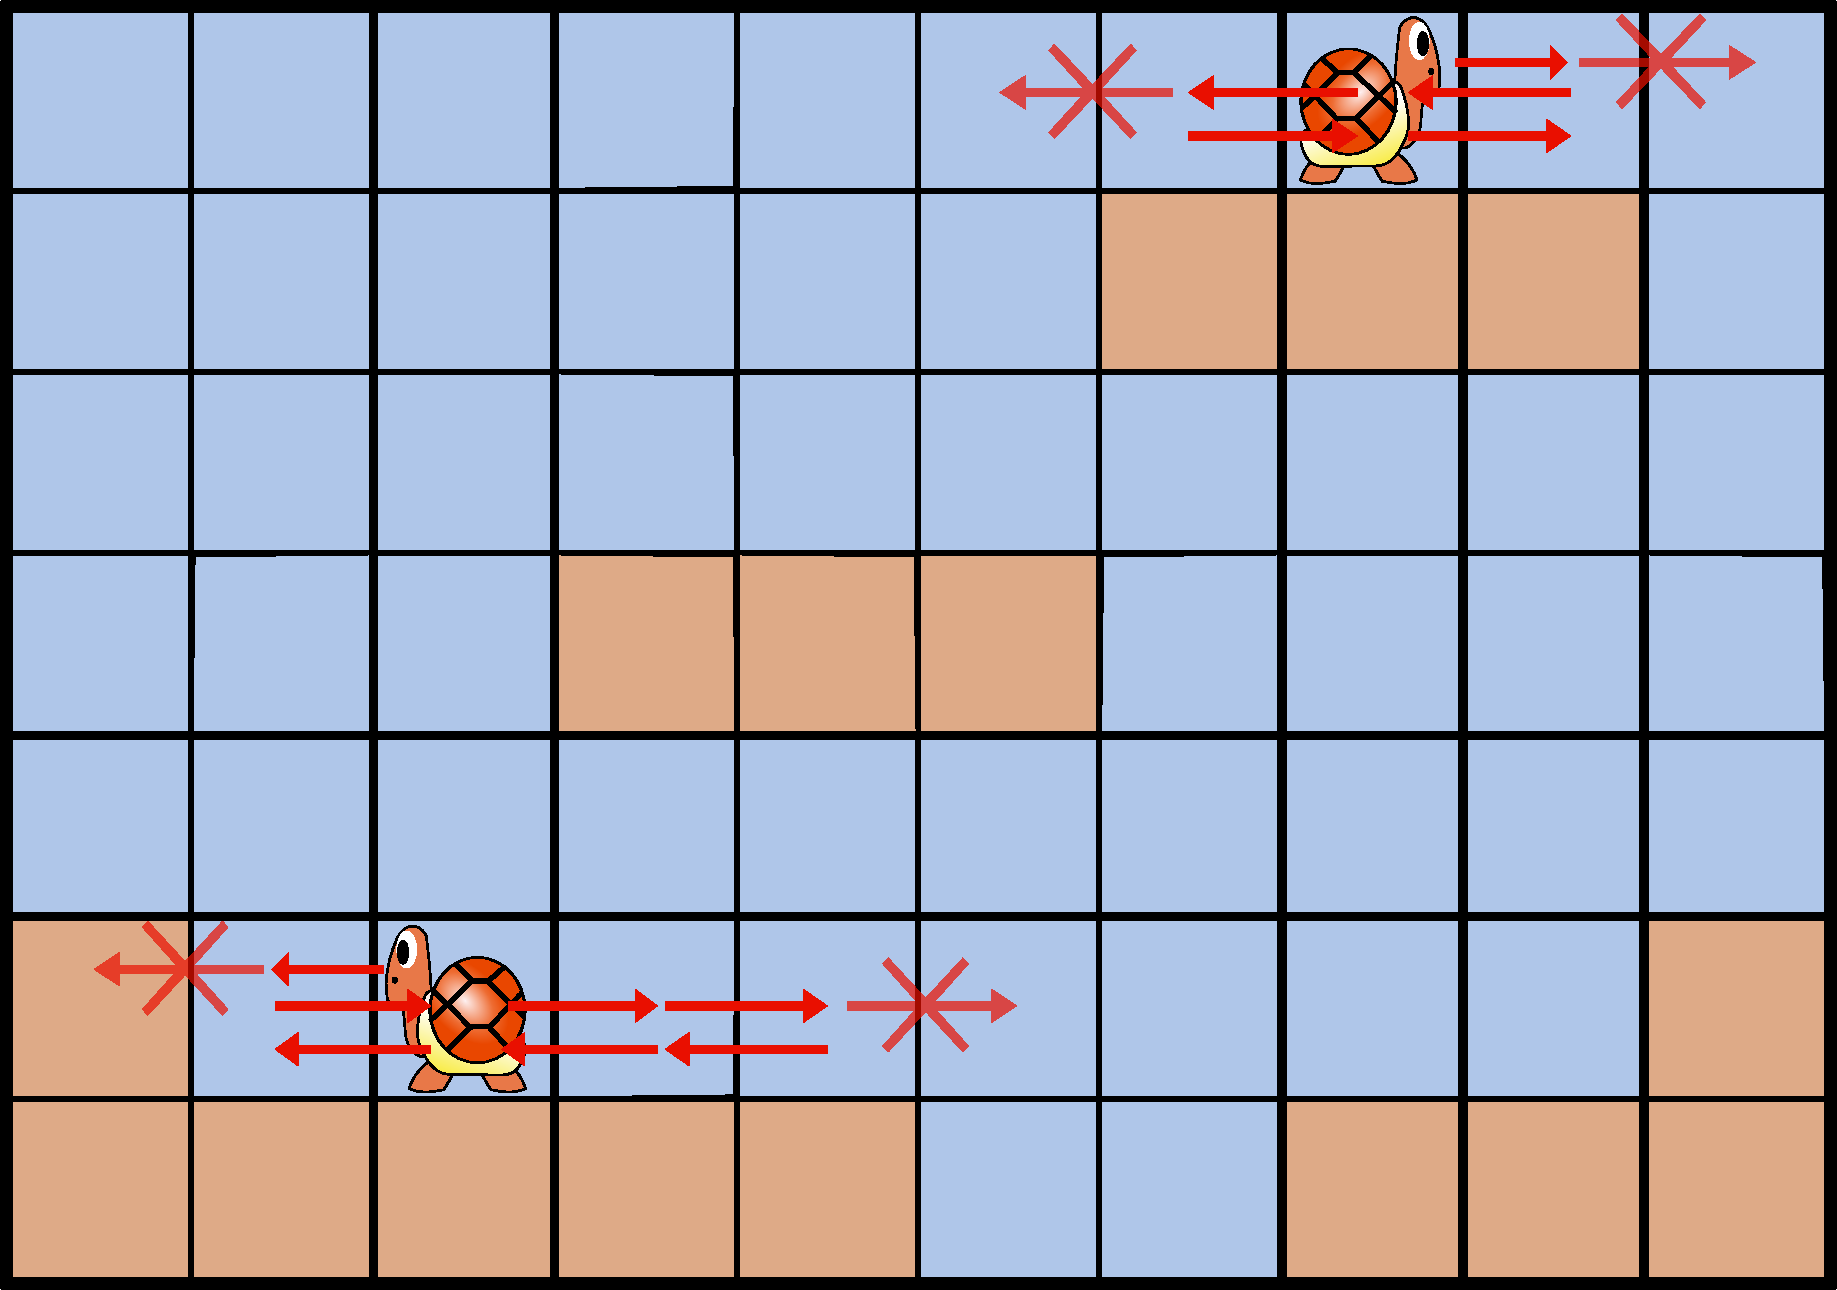
\includegraphics[width=\textwidth]{figures/koopatroopa-red}
  \end{subfigure}
  \begin{subfigure}{0.49\textwidth}
    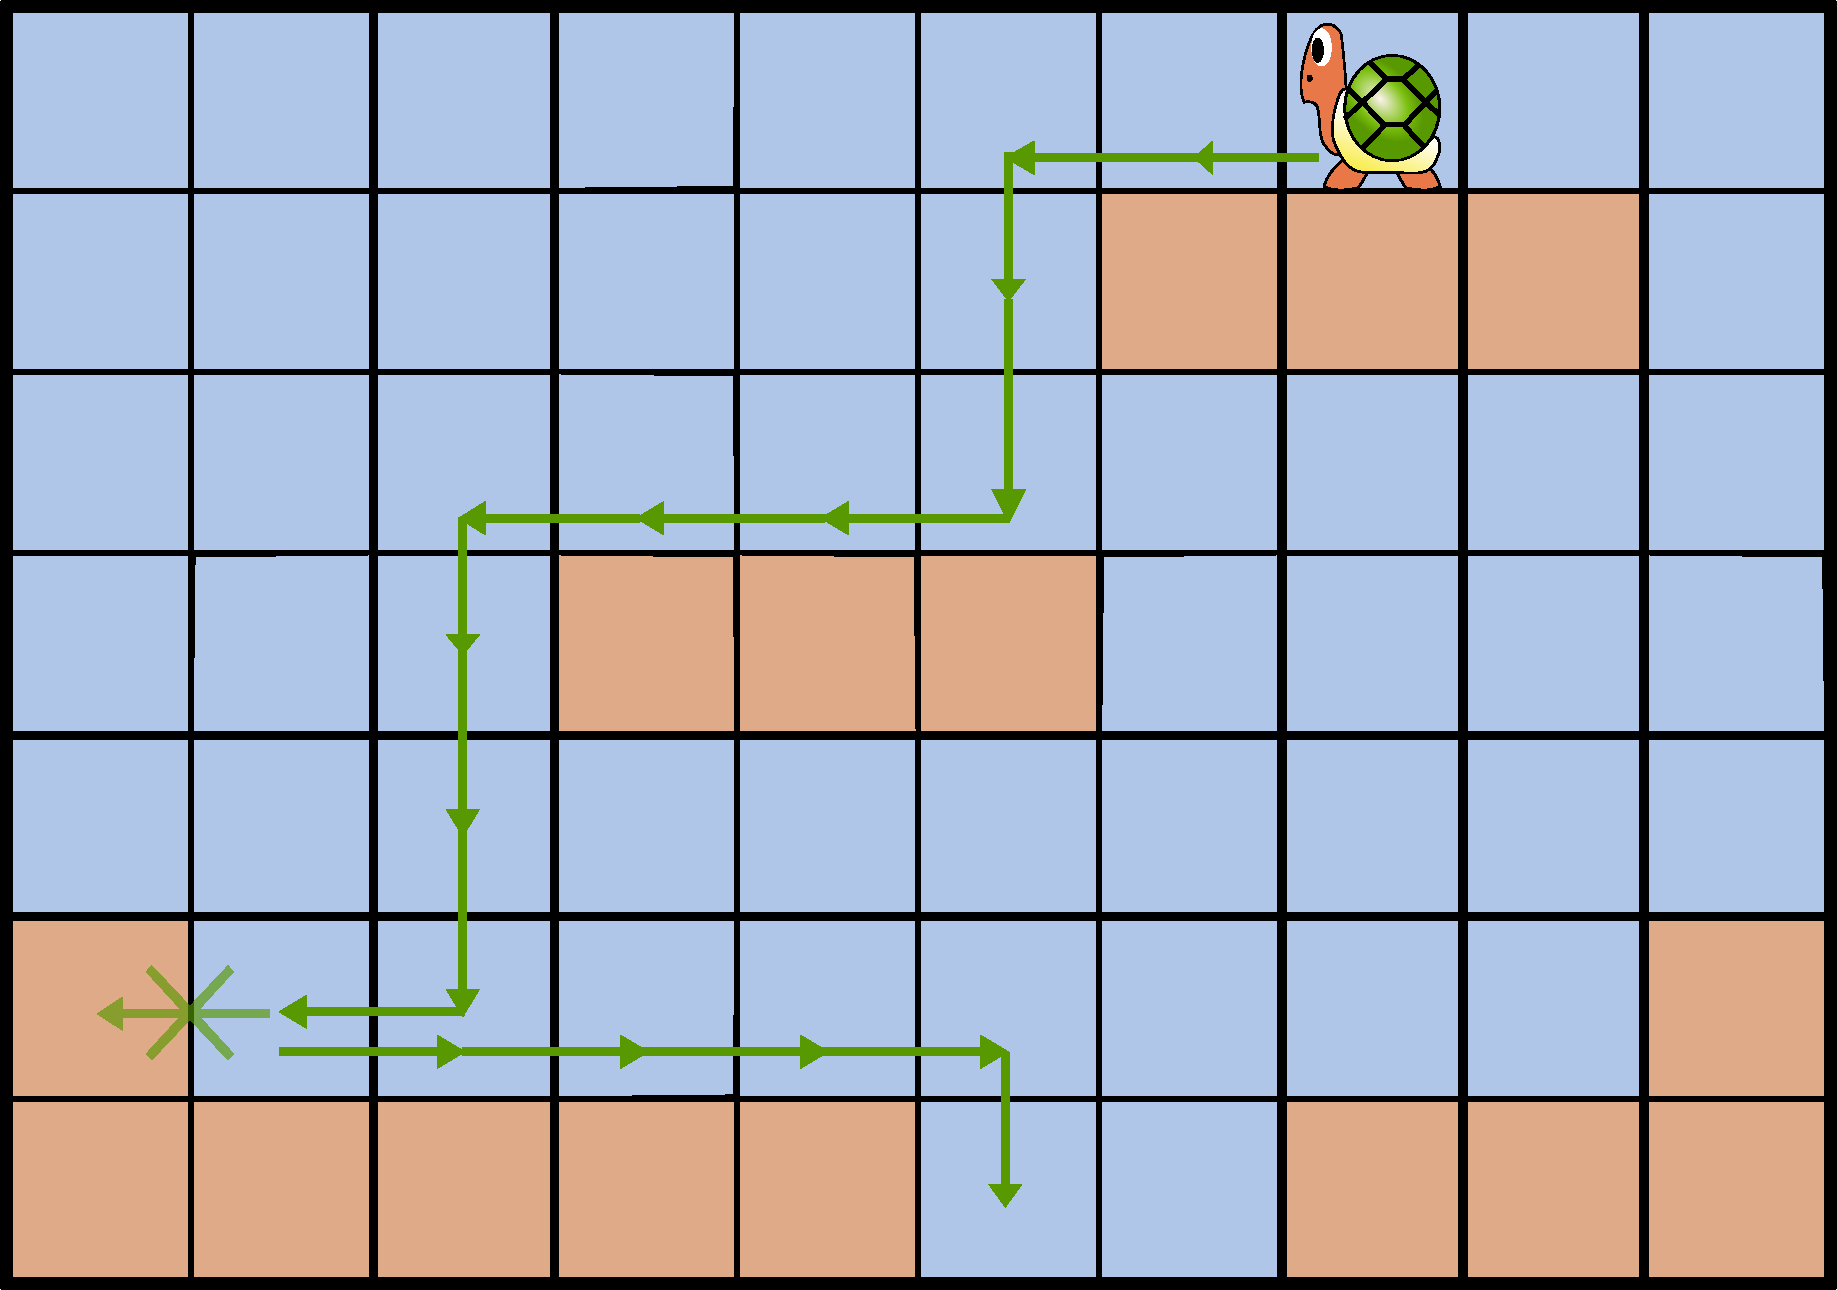
\includegraphics[width=\textwidth]{figures/koopatroopa-green}
  \end{subfigure}
  \caption{Mogelijke paden voor rode en groene Koopa Troopas}
  \label{kooparedgreen}
\end{figure}


\section{Koopa Troopas in Agda}

Om het programmeren met dependent types zo duidelijk mogelijk te illustreren
wordt alle code stap voor stap bekeken in begrijpelijke stukken.  

De code begint met een module declaratie, deze is niet verplicht maar wel
nuttig omdat ze het mogelijk maakt de code te gebruiken in andere programma's.
Daarna importeren we een aantal eenvoudige types uit de standaard bibliotheek.

\inputagda[firstline=8, lastline=15, breaklines]{agda-casestt/koopa.agda}

\iagda{Data.Nat} bevat een unaire voorstelling van natuurlijke getallen die we
gaan gebruiken voor coördinaten. \iagda{Data.Fin} definieert een type voor
begrensde natuurlijke getallen, dit gebruiken we zodat we bij index operaties
niet buiten het bereik van een lijst kunnen gaan. \iagda{Data.Vec} definieert
lijsten met een vaste lengte, vectors dus. \iagda{Data.Unit} definieert een
type, \iagda{⊤} ook wel top genoemd, met één waarde namelijk \iagda{tt}. En,
ten laatste, \iagda{Data.Empty} definieert een leeg type, \iagda{⊥} ook wel
bottom genoemd, waarvoor dus geen waarden bestaan. Dit is anders dan in Haskell
waar je eigenlijk geen leeg type kunt hebben, elk type bevat daar minstens
bottom, wat verschillende dingen kan betekenen, bijvoorbeeld niet eindiging of
een error.

Het volgende stuk is een geneste module declaratie waarin het type
\iagda{Matrix} wordt gedefinieerd als een vector van vectoren en een functie
die een element uit een \iagda{Matrix} projecteert. \iagda{Matrix} is een
inductive family zoals eerder besproken. Omdat \iagda{Matrix} hier gedefinieerd
is als een vector van vectoren kunnen we voor de \iagda{lookup} functie de
\iagda{lookup} functies voor vectoren gebruiken. De volgorde van de indices
speelt hierbij een rol maar omdat de indices van het type \iagda{Fin n}
zijn, kan Agda een fout geven als we ze omwisselen. Vervolgens wordt de module
geopend zodat we het type en de functie kunnen gebruiken zonder de namen te
moeten kwalificeren met de naam van de module.

\inputagda[firstline=17, lastline=23, breaklines]{agda-casestt/koopa.agda}

Hierna begint de oplossing van het probleem eigenlijk pas echt. We definiëren
een aantal types waarmee we de Koopa Troopas en de levels kunnen voorstellen.

\inputagda[firstline=25, lastline=30, breaklines]{agda-casestt/koopa.agda}

Koopa Troopas kunnen twee kleuren hebben dus we definiëren een type
\iagda{Color} met een constructor voor elke kleur. Agda laat ons toe om
constructors met hetzelfde type te groeperen als volgt: \iagda{Green Red :
Color}. Het type \iagda{KoopaTroopa} is geïndexeerd op \iagda{Color}, dit wil
dus zeggen dat er een type is voor elke \iagda{Color}. De Constructor maakt
gebruik van de Agda syntax voor mixfix notatie, in dit geval is \iagda{KT} dus
een postfix constructor. De \iagda{_KT} constructor verwacht een
\iagda{Color} en maakt dan een waarde van het type \iagda{KoopaTroopa c} waar
die \iagda{c} dus de waarde van het argument is. Een groene Koopa Troopa kunnen
we dus voorstellen als \iagda{Green KT} en heeft het type \iagda{KoopaTroopa
Green}, later wordt duidelijk waarom het belangrijk is dat de kleur in het type
zit.

Het volgende stuk bevat nog een aantal type declaraties. Hier definiëren we
posities met alle informatie die we later nodig hebben om te bepalen op welke
posities een Koopa Troopa mag staan.

\inputagda[firstline=32, lastline=48, breaklines]{agda-casestt/koopa.agda}

Elke positie is ofwel lucht ofwel vast: grond of muur of iets dergelijks. Het
type \iagda{Material} stelt deze toestanden voor. Het type \iagda{Clearance}
gebruiken we om te bepalen wie of wat waar mag komen. Een positie met
\iagda{Clearance} \iagda{Low} kan door eender welke Koopa Troopa betreden
worden maar een positie met \iagda{Clearance} \iagda{High} kan enkel door
groene Koopa Troopas betreden worden en gebruiken we om posities aan te duiden
waar de enige logische beweging vallen is. De \iagda{Clearance}
\iagda{Ultimate} gebruiken we voor posities waar geen enkele Koopa Troopa mag
komen. Een positie stellen we voor door een record met twee velden voor een
horizontale en een verticale coördinaat, een veld dat het \iagda{Material} van
de positie aangeeft en een veld voor de \iagda{Clearance}. De constructor
\iagda{pos} kunnen we gebruiken om een positie op te stellen, een voorbeeld van
een positie kan dus zijn: \iagda{pos 3 5 gas Low}, let hierbij op dat de
cijfers door Agda begrepen worden als natuurlijke getallen, hiermee kunnen we
ook enkel natuurlijke getallen voorstellen.

Om de Koopa Troopas een \iagda{Clearance} te geven moeten we ze op een of
andere manier differentiëren en het enige dat verschilt tussen de Koopa Troopas
is hun kleur wat dus de meest logische bepalende factor van de
\iagda{Clearance} wordt.

\inputagda[firstline=50, lastline=52, breaklines]{agda-casestt/koopa.agda}

In plaats van groen en rood gelijk te stellen aan respectievelijk een hoge en
een lage \iagda{Clearance}, werkt de constructor \iagda{<red>} voor beide
kleuren terwijl \iagda{<green>} enkel voor groen werkt. Dit zorgt ervoor dat we
later niet moeten zorgen dat overal waar een lage \iagda{Clearance} toegelaten
is ook een hoge \iagda{Clearance} toegelaten is, een groene Koopa Troopa krijgt
gewoon de \iagda{Clearance} die hij nodig heeft. We zien hier ook dat de mixfix
notatie even goed voor types te gebruiken is, in dit geval gebruiken we dit om
het type voor te stellen als een pijl, \iagda{_c>_}, van een kleur naar een
\iagda{Clearance}.

De volgende twee definities zijn eigenlijk het belangrijkste deel van de
oplossing en steunen op alle voorgaande concepten.

\inputagda[firstline=54, lastline=61, breaklines]{agda-casestt/koopa.agda}

Het \iagda{_follows_⟨_⟩} type is op het eerste zicht waarschijnlijk een beetje
vreemd, dit is omdat de waarden van het type eigenlijk minder belangrijk zijn
dan het type zelf. Het type drukt uit welke positie kan volgen op welke positie
rekening houdend met een kleur. Omdat hier de types van de constructors
belangrijk zijn, overlopen we ze een voor een. \iagda{stay} drukt uit dat een
Koopa Troopa altijd kan blijven staan zolang hij in lucht staat met een lage
\iagda{Clearance}. De \iagda{Material} moet \iagda{gas} zijn omdat een Koopa
Troopa niet in grond of muren mag staan en de \iagda{Clearance} moet
\iagda{Low} zijn omdat we willen dat ook rode Koopa Troopas kunnen stilstaan.
Eigenlijk is stilstaan niet echt een nodige \emph{beweging} maar hiermee kunnen
we later de eindpositie van een pad expliciet maken. De volgende twee
constructors \iagda{next} en \iagda{back} bekijken we tegelijk omdat ze heel
gelijkaardig zijn. Ze drukken uit dat een positie met een bepaalde
\iagda{Clearance} enkel kan volgen op een horizontaal vorige, respectievelijk
volgende, positie als de kleur van de Koopa Troopa die \iagda{Clearance}
oplevert. Ook moet de voorgaande positie een lage \iagda{Clearance} hebben, dit
is omdat we de hoge \iagda{Clearance} gebruiken voor posities waar de enige
mogelijke beweging vallen is. Het \iagda{Material} voor de posities moet nog
steeds \iagda{gas} zijn omdat Koopa Troopas niet in muren kunnen lopen.  De
laatste constructor is \iagda{fall} en die kan enkel gebruikt worden als
beweging van een positie met een hoge \iagda{Clearance}. Aangezien enkel groene
Koopa Troopas op een positie met een hoge \iagda{Clearance} kunnen geraken,
zijn dat ook de enige die kunnen vallen. Nogmaals kunnen we alleen vallen van
een positie in lucht naar een positie in lucht, Koopa Troopas kunnen dus niet
de grond in vallen.

\inputagda[firstline=64, lastline=69, breaklines]{agda-casestt/koopa.agda}

Het type waarmee we de paden voorstellen die Koopa Troopas kunnen afleggen,
\iagda{Path}, moet ervoor zorgen dat enkel geldige paden worden opgesteld voor
een bepaalde Koopa Troopa. De parameter voor de kleur is impliciet omdat die
volgt uit het type van de Koopa Troopa, verder hangt de geldigheid van een pad
af van de Koopa Troopa en kan een pad maar voor één Koopa Troopa tegelijk
opgesteld worden dus is er een parameter waar we een Koopa Troopa verwachten.
Een pad gaat van een beginpositie naar een eindpositie en die moeten kunnen
variëren voor de verschillende constructors dus dat zijn indices. De
constructor voor een leeg pad, \iagda{[]}, moet een begin- en een eindpositie
hebben maar die kunnen we impliciet verkrijgen uit de vorige positie van het
pad en als er geen vorige positie is uit het verwachte type op de plaats waar
we de constructor gebruiken. De constructor om langere paden op te stellen
maakt weer gebruik van mixfix notatie, de \iagda{infixr} declaratie zorgt
ervoor dat de constructor rechts associatief is waardoor we minder haakjes
zullen nodig hebben. De constructor verwacht een positie \iagda{p}, een pad van
\iagda{q} naar \iagda{r}, \iagda{qs}, en een bewijs dat \iagda{q} kan volgen op
\iagda{p} voor de kleur van de Koopa Troopa en resulteert in een pad van
\iagda{p} naar \iagda{r}. \iagda{_↠⟨_⟩_} behoudt de geldigheid van een pad door
het argument van het type \iagda{_follows_⟨_⟩} en de enige manier om een pad te
beginnen is met een leeg pad dat sowieso geldig is. Door deze eigenschappen
zijn alle paden geldig bij wijze van constructie.

We kunnen nu paden beginnen opstellen maar een belangrijk probleem is nog dat
de geldigheid van de paden afhangt van een goede bepaling van de
\iagda{Clearance} van elke positie. Wat volgt is eerst een klein voorbeeld van
een pad en daarna een mogelijke oplossing voor een juiste bepaling van de
\iagda{Clearance} voor elke positie.

\inputagda[firstline=71, lastline=74, breaklines]{agda-casestt/koopa.agda}

Om ervoor te zorgen dat de \iagda{Clearance} juist bepaald wordt, gaan we
een functie gebruiken die de regels voor de bepaling van de \iagda{Clearance}
van een positie uitdrukt.

\inputagda[firstline=78, lastline=86, breaklines]{agda-casestt/koopa.agda}

De \iagda{matterToPosVec} functie verwacht twee vectoren van dezelfde lengte
met \iagda{Material}s in en twee coördinaten die aangeven bij welke positie het
eerste \iagda{Material} in de eerste vector hoort. Het resultaat is een vector
van dezelfde lengte met posities in met de juiste coördinaten, de
\iagda{Material}s uit de eerste vector en de juiste \iagda{Clearance} die
afhangt van het \iagda{Material} van de positie onder een positie, vandaar dat
we twee vectoren in de invoer nodig hebben. Het basisgeval is wanneer de
vectoren leeg zijn, in het andere geval bepaalt de functie \iagda{clearance}
wat de juiste \iagda{Clearance} voor de positie is aan de hand van het
\iagda{Material} van de positie zelf en van de positie er onder. Lucht boven
lucht heeft \iagda{Clearance} \iagda{High} omdat daar alleen gevallen kan
worden, lucht boven grond heeft \iagda{Clearance} \iagda{Low} omdat elke Koopa
Troopa moet kunnen staan. Alle grond en muur posities hebben \iagda{Clearance}
\iagda{Ultimate} omdat geen enkele Koopa Troopa zich in een muur of in de grond
mag bevinden.

Door vectoren te geven van alle \iagda{Material}s op een horizontale rij en de
rij daaronder kunnen we nu de \iagda{Clearance}s juist bepalen. Voor de
voorstelling van een level kunnen we dus een vector van zulke vectoren
gebruiken. Uiteindelijk willen we een matrix van posities die het level
voorstelt maar omdat het voor de recursie beter uitkomt als we met een vector
van vectoren werken voor de invoer, gebruiken we geen matrix voor de invoer.

\inputagda[firstline=88, lastline=98, breaklines]{agda-casestt/koopa.agda}

De functie \iagda{matterToPosVecs} maakt gebruik van de vorige functie om een
vector van vectoren van \iagda{Material}s om te zetten in een vector van
vectoren van posities. Het basisgeval is de lege vector en die wordt omgezet in
een lege vector. In het recursieve geval zien we dat de \iagda{_∷_} constructor
voor vectoren gebruikt wordt in de prefix vorm, dit is omdat we willen pattern
matchen op een derde impliciet argument en drie argumenten gaan niet goed samen
met een binaire infix constructor. We gebruiken \iagda{matterToPosVec} op de
eerste vector in de vector van vectoren en op de vector daaronder, die we
verkrijgen uit de functie \iagda{unders}. \iagda{unders} is eigenlijk heel
gelijkaardig aan de \iagda{head} functie maar is specifieker voor een vector
van vectoren en heeft een \emph{fallback} argument dat we teruggeven als we de
rij onder de laatste rij nodig hebben. Het enige dat dan nog rest is om de
recursieve oproep te doen op de rest van de vector van vectoren. De
\iagda{matsToMat} functie maakt van de vector van vectoren van posities, die we
terugkrijgen uit \iagda{matterToPosVecs}, een matrix waarbij de rijen eerst van
volgorde gewisseld worden omdat de index $(0,0)$ bij een matrix linksboven zit
en in de levelvoorstelling links onder.

Met deze functies kunnen we gemakkelijk een level opstellen door de juiste
\iagda{Material}s in de juiste volgorde op te geven, hierbij wordt dan meteen
de juiste \iagda{Clearance} bepaalt voor elke positie. Om onze notatie iets
visueler te maken definiëren we nog twee functies met een unicode symbool.

\inputagda[firstline=100, lastline=114, breaklines]{agda-casestt/koopa.agda}

De functies \iagda{□_} en \iagda{■_} zijn gewoon afkortingen voor
respectievelijk een vector die begint met \iagda{gas} en nog een staart
verwacht en een vector die begint met \iagda{solid} en nog een staart verwacht.
Deze functies zijn gedefinieerd met een underscore ook al zijn ze gewoon prefix
functies omdat de \iagda{infixr} declaratie enkel van toepassing is op mixfix
functies. Zoals we kunnen zien is het level, dat tevens in figuur
\ref{kooparedgreen} te zien is, redelijk herkenbaar ook al stellen we het
gewoon voor met tekst, dit is een voordeel van werken met de volledige unicode
karakterset.

Het enige dat ons nu nog rest te definiëren zijn een aantal hulp functies om
natuurlijke getallen om te zetten in getallen van het type \iagda{Fin n} omdat
we die niet met cijfers kunnen schrijven.

\inputagda[firstline=116, lastline=130, breaklines]{agda-casestt/koopa.agda}

De eerste functie, \iagda{_<'_}, vergelijkt twee natuurlijke getallen en geeft
een type terug, in een taal waar types geen waarden zijn gaat dit meestal niet.
Als het eerste getal strikt kleiner is dan het tweede is dit type \iagda{⊤},
anders is het type \iagda{⊥}. Een element van het type \iagda{⊤} kan altijd
impliciet ingevuld worden, er is er namelijk maar één: \iagda{tt}. Een element
van het type \iagda{⊥} kan nooit gegeven worden want er zijn er geen.
Van deze functie maken we gebruik in het type van \iagda{fromNat}, een functie
die een natuurlijk getal omzet in een element van \iagda{Fin n}. We kunnen een
natuurlijk getal \iagda{k} maar omzetten in een \iagda{Fin n} als \iagda{k}
strikt kleiner is dan \iagda{n}. Het type \iagda{k <' n} is ofwel gelijk aan
het type \iagda{⊤} ofwel aan het type \iagda{⊥}, in het eerste geval moeten we
dus geen expliciete waarde geven, in het tweede geval kunnen we geen waarde
geven en dus kunnen we de functie ook niet oproepen met een \iagda{k} die we
nooit kunnen omzetten in een \iagda{Fin n}. Op deze manier kan de typechecker
ons waarschuwen wanneer we dit ergens wel proberen doen. In deze functie zien
we nog iets nieuws, de eerste vergelijking heeft geen rechterzijde. Dit is
omdat er geen waarde bestaan van het type \iagda{Fin n}, dat isomorf is met het
type \iagda{⊥}. Omdat de \iagda{n} in \iagda{Fin n} een natuurlijk getal is, is
\iagda{0} niet uitgesloten en omdat Agda een totale programmeertaal is moeten
we voor elke mogelijke waarde van het argument \iagda{n} een antwoord bieden.
In dit geval is het type \iagda{k <' n} sowieso gelijk aan \iagda{⊥} en omdat
we geen waarde van dat type kunnen krijgen kunnen we gebruik maken van het
zogenaamde \emph{absurd} pattern: \iagda{{}} of \iagda{()}. Het absurd pattern
geeft aan dat er onmogelijk een waarde van het juiste type bestaat, de
typechecker moet dit wel kunnen nagaan dus dit werkt alleen voor types die
eenvoudig genoeg zijn. Als Agda overtuigd is dat er geen waarde bestaat, moeten
we ook geen rechterzijde opgeven. In de derde vergelijking zien we nog dat het
\emph{bewijs} dat \iagda{k} kleiner is dan \iagda{n} expliciet doorgegeven
wordt en dus geldig blijft voor het recursieve geval, het is tenslotte ook maar
een eenvoudige waarde, \iagda{tt}. De functie \iagda{f} is slechts een
afkorting voor \iagda{fromNat}. De functie \iagda{p} is een afkorting voor
\iagda{lookup} waarbij de coördinaten omgewisseld zijn voor de leesbaarheid en
het level niet moet opgegeven worden omdat dat in alle voorbeelden hetzelfde
is.

Met al deze extra definities kunnen we nu paden op een compacte manier
definiëren zoals we in de rest van de voorbeelden zien.

\inputagda[firstline=132, lastline=144, breaklines]{agda-casestt/koopa.agda}

\iagda{red_path_one} en \iagda{red_path_two} stellen de paden voor die door de
rode Koopa Troopas afgelegd wordt in figuur \ref{kooparedgreen}, het vakje
linksonder heeft coördinaat $(0,0)$, de x-as loopt horizontaal en de y-as
verticaal. Voorbeelden van paden waar niets mis mee is zijn eigenlijk niet zo
interessant, die kunnen in het originele spel ook voorgesteld worden. Het wordt
pas interessant als we proberen om een ongeldig pad op te stellen want dat is
wat we proberen te voorkomen.

\inputagda[firstline=1, lastline=12, breaklines]{agda-casestt/koopa-errors.agda}

De fout bij \iagda{red_nopath_one} ziet eruit als volgt:

%----------------------------------------%
\begin{minted}[fontsize=\small]{agda}
  gas != solid of type Material
  when checking that the expression stay has type
  pos 0 (suc zero) gas Low follows p (f 0) (f 1) ⟨ Red ⟩
\end{minted}

Agda geeft aan dat de positie in het type van \iagda{stay} niet overeenkomt met
de positie, door \iagda{stay} te gebruiken op positie $(0,1)$ zou het type
\iagda{pos 0 1 solid Ultimate follows pos 0 1 solid Ultimate ⟨ Red ⟩} moeten
zijn maar dat is niet toegelaten in de definitie van de constructor.
Eigenlijk verwachten we een fout daar waar we een muur in lopen en hier krijgen
we de fout pas te zien als we al in een muur staan. Dit is omdat de
\iagda{_↠⟨_⟩_} constructor rechts associatief is, dus de eerste fout die Agda
tegenkomt zit zo ver mogelijk vanachter in het pad.

In de fout voor \iagda{red_nopath_two} kunnen we zien dat de beweging waarbij
we een muur zouden inlopen wel als fout wordt gezien:

%----------------------------------------%
\begin{minted}[fontsize=\small]{agda}
  gas != solid of type Material
  when checking that the expression p (f 1) (f 1) ↠⟨ back ⟩ [] has
  type Path (Red KT) (p (f 1) (f 1)) (p (f 0) (f 1))
\end{minted}

Deze fout is zo goed als hetzelfde als de vorige, alleen gaat het nu om de
\iagda{back} constructor en is de expressie waar de fout zich bevindt niet even
ver gereduceerd omdat het type van \iagda{back} ingewikkelder is.

Een pad voor een rode Koopa Troopa moet ook ongeldig zijn als een Koopa Troopa
zou vallen bij het afleggen van het pad:

%----------------------------------------%
\begin{minted}[fontsize=\small]{agda}
  Low != High of type Clearance
  when checking that the expression p (f 4) (f 1) ↠⟨ next ⟩ [] has
  type Path (Red KT) (p (f 4) (f 1)) (p (f 5) (f 1))
\end{minted}

Als een rode Koopa Troopa van een afgrond afloopt, is het niet het
\iagda{Material} dat in de weg zit, het is namelijk allemaal lucht, maar wel
het feit dat een rode Koopa Troopa niet de juiste \iagda{Clearance} heeft.

Voor een groene Koopa Troopa kunnen we opnieuw geldige paden opstellen:

\inputagda[firstline=159, lastline=184, breaklines]{agda-casestt/koopa.agda}

In \iagda{green_path_one} zien we één van de geldige paden voor rode Koopa
Troopas terugkomen. Een pad dat geldig is voor een rode Koopa Troopa is ook
geldig voor een groene Koopa Troopa. In het oorspronkelijke spel zijn Koopa
Troopas ook obstakels voor elkaar, op die manier zou een groene Koopa Troopa
dus beperkt kunnen worden tot een pad dat een rode ook kan afleggen. Evenzeer
is een pad voor een rode Koopa Troopa dat omkeert voor er een obstakel in de
weg zit, mogelijk. Opnieuw kan dit nuttig zijn, bijvoorbeeld om de Koopa
Troopas actief de speler te laten achtervolgen als die in de buurt komt,
waarbij ze dus vroeger dan nodig omkeren. In \iagda{green_path_two} zien we het
langere pad dat in figuur \ref{kooparedgreen} geïllustreerd is.

Voor een groen Koopa Troopa is het geen fout als het pad van een afgrond af
gaat en dan naar beneden valt. Maar er treedt zoals verwacht nog wel een fout
op als we proberen een muur in te lopen:

\inputagda[firstline=14,lastline=16,breaklines]{agda-casestt/koopa-errors.agda}

%----------------------------------------%
\begin{minted}[fontsize=\small]{agda}
  gas != solid of type Material
  when checking that the expression p (f 1) (f 1) ↠⟨ back ⟩ [] has
  type Path (Green KT) (p (f 1) (f 1)) (p (f 0) (f 1))
\end{minted}

Deze fout is identiek aan die voor \iagda{red_nopath_two}. In het volgende
deel bespreken we de implementatie van dit model in Haskell.


\section{Koopa Troopas in Haskell}

In Haskell beginnen we de code met de LANGUAGE pragma's die besproken zijn in
hoofdstuk \ref{ch:agda-haskell}. Daarna komt de module declaratie, hier zien we
voor de eerste keer dat Haskell redelijk strikte regels heeft over naamgeving,
modules types en constructors moeten met een hoofdletter beginnen en functies
met een kleine letter.

\inputhaskell[firstline=8, lastline=11, breaklines]{haskell-casestt/koopa.hs}

Om te beginnen moeten we een aantal types die we in Agda uit de standard
library kunnen halen zelf implementeren or is bijvoorbeeld geen erg grote nood
aan een unaire voorstelling van natuurlijke getallen in Haskell. De naamgeving
en technieken die we hier gebruiken komen uit een artikel \ref{hasochism} over
dependently typed programmeren in Haskell met de titel: "Hasochism: The
Pleasure and Pain of Dependently Typed Haskell Programming." Het wordt redelijk
snel duidelijk waarom het artikel die titel heeft.

\inputhaskell[firstline=13, lastline=24, breaklines]{haskell-casestt/koopa.hs}

We beginnen met het definiëren van onze unaire natuurlijke getallen, dankzij de
datatype promotion van de DataKinds extensie hebben we nu ook meteen unaire
natuurlijke getallen op het typeniveau. Wat we nog missen is een verbinding
tussen waarden op het waardeniveau en waarden op het typeniveau zoals die er
wel is in Agda, daar kunnen we een argument van de functie ook in het type
gebruiken. In Haskell kunnen we dit niet echt doen maar we kunnen het wel
imiteren met een zogenaamde singleton constructie. Dit zien we in de definitie
van \ihask{Natty n}, elke waarde die we opstellen heeft een ander type:
\ihask{Zy} heeft type \ihask{Natty Z} en \ihask{Sy Zy} heeft type \ihask{Natty
(S Z)}. Omdat elk type \ihask{Natty n} maar één waarde bevat, heeft deze
constructie de benaming singleton gekregen. De functie \ihask{natter}, ongeveer
te lezen als "meer Nat-achtig," zet een \ihask{Natty n} om in een \ihask{Nat},
hierbij werpen we als het ware informatie op het typeniveau weg. De omgekeerde
conversie gaat niet zomaar, er is geen manier om statisch te bepalen wat de
\ihask{n} in het return type \ihask{Natty n} zou moeten zijn. Om dit bij
benadering toch te kunnen doen hebben we een derde type nodig, \ihask{NATTY}.
Dit type verstopt als het ware de typeniveau informatie van een \ihask{Natty
n}. Nu kunnen we de functie \ihask{nattyer}, "meer Natty-achtig," wel
schrijven. De definitie is eenvoudig, in het recursieve geval moeten we een
pattern match doen op de recursieve oproep om met de eigenlijke waarde van de
\ihask{Natty n} te kunnen werken.

Haskell ontbreekt logischerwijs tevens een type voor begrensde natuurlijke
getallen. Deze keer kunnen we de extra types niet definiëren omdat Haskell het
\ihask{Fin n} type niet kan promoveren. De DataKinds extensie promoveert enkel
types met argumenten met kind \ihask{*}.

\inputhaskell[firstline=27, lastline=35, breaklines]{haskell-casestt/koopa.hs}

De definitie voor \ihask{Fin n} is identiek aan die uit de Agda standard
library voor zover dat mogelijk is. De functie \ihask{intToFin} dient ongeveer
hetzelfde doel als de \iagda{fromNat} functie uit de Agda code. Omdat Haskell
geen cijfers toelaat voor natuurlijke getallen, vertrekken we van het
\ihask{Integer} type. Dit brengt met zich mee dat we negatieve getallen
toelaten, hiervoor werpen we gewoon een fout op.

Vervolgens is er het type \ihask{Vec} dat ook weer logischerwijs niet in
Haskell aanwezig is met de bijhorende functies.

\inputhaskell[firstline=38, lastline=58, breaklines]{haskell-casestt/koopa.hs}

Haskell laat binaire infix constructors toe door hun naam te beginnen met een
dubbelpunt, toevallig kunnen we zo bijna dezelfde notatie gebruiken als in
Agda. \ihask{vlookup} haalt een element uit een vector met behulp van een
begrensd getal dus we sluiten uit dat een index te groot of te klein is.
\ihask{vreplicate} stelt een vector op met een bepaald aantal herhalingen van
een element, we hebben hier een \ihask{Natty n} nodig omdat we de waarde
\ihask{n} moeten kennen voor het type van de vector die we willen teruggeven.
\ihask{vreverse} keert de volgorde van de elementen in een vector om.

Nu kunnen we ook het \ihask{Matrix} type definiëren. Dit type en de voorgaande
types zijn niet gedefinieerd in submodules zoals we \iagda{Matrix} gedefinieerd
hebben in Agda omdat Haskell geen concept heeft van submodules. We zouden deze
types allemaal in modules in hun eigen bestanden kunnen definiëren maar omdat
het weinig code is en slechts tot voorbeeld dient, is dit achterwege gelaten.

\inputhaskell[firstline=61, lastline=65, breaklines]{haskell-casestt/koopa.hs}

Zowel het \ihask{Matrix} type als de \ihask{mlookup} functie gelijken sterk op
hun tegenhangers in Agda. Het grootste verschil is dat we in Haskell met
polymorfisme werken daar waar we in Agda gewoonlijk impliciete argumenten
gebruiken.



\chapter{Case: Verified Red-Black Trees}
\label{case:rbtree}


\section{Inleiding}

Deze tweede gevalstudie gaat over een implementatie van red-black trees
\cite{rbtrees}. Red-black trees zijn een soort binaire zoekbomen, door één
extra bit aan informatie bij te houden voor elke knoop zijn ze bij benadering
gebalanceerd. Deze benaderende balans is goed genoeg om $\mathcal{O}(\log{}n)$
tijdscomplexiteit te garanderen voor: het opzoeken van een element, een element
toe te voegen en een element te verwijderen. Zoekbomen worden vaak gebruikt om
meer abstracte datastructuren te implementeren, bijvoorbeeld verzamelingen en
associatieve arrays. Vooral voor de geordende varianten van die datastructuren
kunnen zoekbomen voordeliger zijn voor de implementatie dan hashtabellen omdat
zoekbomen per definitie geordend zijn.

Chris Okasaki heeft een elegante implementatie van red-black trees
\cite{okasaki} in een functionele programmeertaal geschreven, in Haskell.
De implementaties in dit hoofdstuk zijn hierop gebaseerd.
Zijn implementatie is gebaseerd op een bondige formulering van de red-black
tree invarianten. Deze gaan als volgt:

\begin{description}
  \item[Invariant 1] Geen enkele rode knoop heeft een rode ouder.
  \item[Invariant 2] Elk pad van de wortel naar een blad bevat hetzelfde aantal
                     zwarte knopen.
\end{description}

De implementatie van Okasaki wordt hier herhaald zodat het eenvoudig is om te
zien wat van het oorspronkelijk algoritme komt en wat toegevoegd is om de twee
invarianten statisch te garanderen.

\inputhaskell[breaklines]{haskell-casestt/Okasaki.hs}

Omdat deze implementatie zo kort en eenvoudig is kan bijna iedereen deze code
waarschijnlijk begrijpen. Maar omdat datastructuren zo fundamenteel zijn aan
alles wat programma's doen, is het belangrijk dat ze correct zijn. Eén
datastructuur kan nog wel correct gehouden worden door goed na te denken over
aanpassingen en een mentaal model van de werking bij te houden maar vanaf dat
er een tiental datastructuren zijn, is er bijna niemand die ervoor kan zorgen
dat die correct zijn en blijven. Gewoonlijk wordt er daarom een suite van tests
opgesteld die regelmatig uitgevoerd dienen te worden, iedere keer dat er een
fout gevonden wordt, worden er tests toegevoegd die die fout zouden detecteren
als ze ooit terugkomt. Dit is een bewezen methode maar omvat onmiskenbaar een
hoop extra werk: tests moeten geschreven worden en onderhouden omdat
bijvoorbeeld de interface tot het programma kan veranderen. Een zwakheid van
deze aanpak is dat de tests vaak niet alle mogelijke gevallen afdekken: we
moeten vertrouwen op ons vermogen om te redeneren over de code om speciale
gevallen te ontdekken waar een grote kans voor bestaat dat er iets mis gaat. Om
dit op te lossen zijn er gerandomiseerde testprogramma's zoals QuickCheck
\cite{quickcheck} bedacht, die het vinden van speciale gevallen automatiseren.
In de implementaties in dit hoofdstuk daarentegen maken we gebruik van de
expressiviteit van dependent types om de invarianten door het typesysteem te
laten nakijken en zo de code statisch te verifiëren.


\section{Red-Black Trees in Agda}

De code van Okasaki is heel elegant maar ze bevat heel weinig statische
garanties. Het \ihask{Tree} type bijvoorbeeld voorkomt helemaal geen misbruik:
\ihask{T R (T R E 1 E) 2 E} is een geldige boom, net zoals \ihask{T B (T B E 1
E) 2 E} terwijl beiden niet voldoen aan de invarianten van red-black trees.
Dit betekent dat we goed moeten opletten als we een functie schrijven die een
\ihask{Tree} moet teruggeven omdat we geen waarschuwing krijgen als we een
ongeldige boom proberen op te stellen. Om nog maar niet te vermelden hoe we met
ongeldige bomen als invoer moeten omspringen? De gemakkelijkste oplossing is om
er niets aan te doen, maar dan kan het programma crashen omdat we ergens in een
functie impliciet aannamen dat de invoer een geldige red-black tree zou zijn.
Wat mogelijk nog erger is dan een crash is geen crash, een ongeldige boom gaat
door het programma en elke functie waarmee die in aanraking komt kan er iets
aan verandert hebben, op het einde merken we dat de uitvoer niet correct is
en nu moeten we uitzoeken waar het precies mis gegaan is. De expressiviteit van
dependent types kan ons hierbij helpen, als we ervoor zorgen dat een ongeldige
boom niet opgesteld kan worden, kunnen we ook geen problemen hebben met
ongeldige bomen. Het \iagda{Tree} type in Agda is eigenlijk een exacte
definitie van wat een red-black tree is terwijl het \ihask{Tree} type van
Okasaki eender welke binaire boom met rood en zwart gekleurde knopen voorstelt.

\inputagda[firstline=16,lastline=33,breaklines]{agda-casestt/RedBlackTree.agda}

We beginnen met een aantal imports en de definities van implicatie en mixfix
\emph{if then else}, alles dat we hier zien wordt uitgelegd daar waar het voor
het eerst gebruikt wordt.

\inputagda[firstline=35,lastline=43,breaklines]{agda-casestt/RedBlackTree.agda}

We definiëren een geparametriseerde module, \iagda{RBTree}, met als parameter
een \emph{record} van het type \iagda{StrictTotalOrder}. De \iagda{a} en
\iagda{ℓ} parameters zijn levels en zorgen ervoor dat de elementen van onze
boom ook elementen van een type in één van de grotere universa kunnen zijn:
\iagda{Set₁}, \iagda{Set₂}, etc.
Door een waarde van het type \iagda{StrictTotalOrder} te eisen, kunnen we er
zeker van zijn dat we de elementen kunnen ordenen en de zoekbomen dus nuttig
kunnen invullen. De twee volgende regels zorgen ervoor dat we in de rest van de
code in de module kunnen verwijzen naar dit type met een strikte totale
orderelatie als \iagda{A}. De \emph{pattern} declaraties zorgen ervoor dat we
met een compactere notatie kunnen werken voor het resultaat van een
vergelijking. Op deze manier verbergen we een aantal bewijzen die we niet echt
nodig hebben. Ten slotte kiezen we een symbool om de vergelijkingsfunctie te
verkorten. Het symbool staat voor de relatie ``kleiner dan of gelijk aan'' maar
het resultaat van de functie is \iagda{LT} als het eerste argument voor het
tweede komt, \iagda{EQ} als de elementen gelijk zijn en \iagda{GT} als het
eerste element na het tweede komt.

Nu kunnen we net als Okasaki beginnen met definiëren wat een kleur is en wat een
red-black tree is.

\inputagda[firstline=46,lastline=59,breaklines]{agda-casestt/RedBlackTree.agda}

Het type \iagda{Color} is heel eenvoudig, de functie \iagda{_=ᶜ_} is niet meer
dan een vergelijking van twee kleuren op gelijkheid met een Booleaans
resultaat. We definiëren ook nog een synoniem voor natuurlijke getallen,
\iagda{Height}, wat het aantal zwarte knopen op een pad van de wortel naar een
willekeurig blad voorstelt. Het type \iagda{Tree} is ook nog redelijk eenvoudig
maar dwingt wel meteen de twee invarianten af. De constructor voor een rode
knoop, \iagda{R}, laat enkel kinderen toe met een zwarte wortel, op die manier
kan een rode knoop nooit een rode ouder hebben. Dit zorgt dat invariant 1
behouden blijft. Overigens moeten de twee kinderen dezelfde hoogte hebben om
invariant 2 te behouden. De constructor, \iagda{B}, eist eveneens dat de
kinderen een gelijke hoogte hebben zodat invariant 2 behouden blijft. Meer is
er niet nodig om een type op te stellen dat enkel correcte red-black trees kan
voorstellen.

Het grootste voordeel van dit preciezere type is tegelijk ook een nadeel:
algoritmes verbreken vaak tijdelijk een of meerdere invarianten omdat het soms
eenvoudiger is om iets kapot te maken en daarna in stappen te herstellen dan om
alles in één keer goed te doen. Dit is vooral het geval wanneer een verandering
een andere verandering tot gevolg kan hebben met een domino-effect. Okasaki
maakt gebruik van deze techniek in zijn \ihask{ins} functie: \ihask{ins} zou
een ongeldige boom kunnen teruggeven en daarom zijn de oproepen naar
\ihask{ins} als het ware afgeschermd door \ihask{makeBlack} of \ihask{balance}.
De \ihask{ins} functie kan een boom teruggeven met een rode wortel en één rood
kind, dit noemen we ook wel een infrarode boom. Een infrarode boom kan altijd
hersteld worden door de wortel zwart te kleuren maar dit vergroot de hoogte met
één. Tijdens het toevoegen van een element vermijden we liever veranderingen
van hoogte omdat als één kind hoger wordt dan het andere, we de boom moeten
herbalanceren. De recursieve oproepen naar \ihask{ins} zijn daarom afgeschermd
door oproepen naar \ihask{balance}. Het is tevens het algoritme voor
herbalancering waar de oplossing van Okasaki zijn elegantie vandaan haalt. Als
het resultaat van een recursieve oproep naar \ihask{ins} een infrarode boom is,
dan moet de wortel van het kind waarin we de waarde hebben toegevoegd, rood
zijn geweest en dat kan alleen als de ouder van dat kind zwart was. Dit zijn nu
net de voorwaarden voor de \ihask{balance} functie van Okasaki. Omdat we zulk
een tijdelijke schending van de invarianten niet kunnen voorstellen in ons
\iagda{Tree} type, hebben we een nieuw type nodig dat infrarode bomen kan
voorstellen.

\inputagda[firstline=61,lastline=63,breaklines]{agda-casestt/RedBlackTree.agda}

Omdat we nu twee verschillende types hebben voor red-black trees en infrarode
bomen kunnen we de \iagda{balance} functie niet implementeren zoals Okasaki.
Soms zou het type van het linker argument infrarood moeten zijn en het rechtse
red-black en soms omgekeerd. We kunnen dit gedrag wel vatten in een nieuw type.

\inputagda[firstline=65,lastline=67,breaklines]{agda-casestt/RedBlackTree.agda}

Dankzij de flexibele mixfix syntax van Agda kunnen we nu deze toepassing uit
Haskell, \ihask{balance B infra b c}, als volgt schrijven in Agda:
\iagda{balance (infra ◂ b ◂ c)}. We hebben ook geen nood meer aan het kleur
argument, waarom komt later aan bod.
We komen nog één type te kort, sommige functies zoals \iagda{ins} kunnen zowel
een geldige als een ongeldige boom teruggeven. Omdat deze voorgesteld worden
door twee aparte types hebben we een type nodig dat werkt als een disjuncte
som van die twee types.

\inputagda[firstline=69,lastline=71,breaklines]{agda-casestt/RedBlackTree.agda}

Meer precisie kost meer werk, wat bij Okasaki één type was, zijn er nu vier.
Hoe preciezer we willen zijn hoe meer we expliciet moeten maken: dit zal ook
duidelijk worden in de implementaties van de functies. De eerste functie die we
bekijken is \iagda{balance}.

\inputagda[firstline=75,lastline=79,breaklines]{agda-casestt/RedBlackTree.agda}

De implementatie gelijkt sterk op die van Okasaki maar er zijn subtiele
verschillen. Het kleur argument is niet langer nodig, Okasaki gebruikt dit
eigenlijk alleen in het geval dat hij niets doet met de invoer om de argumenten
terug samen te stellen tot een geldige boom met dezelfde kleur wortel. Omdat
onze functie enkel bomen aanvaard die gebalanceerd \emph{moeten} worden en een
gebalanceerde boom altijd rood is, weten we op voorhand wat de kleur van de
boom is die we teruggeven. Dit kunnen we alleen maar doen omdat ons type nu
strikt genoeg is om geldige bomen uit te sluiten van \iagda{balance}. Dit
betekent wel dat we op de plaats waar we \iagda{balance} willen gebruiken,
zeker moeten zijn dat we een ongeldige boom hebben. Om die beslissing te kunnen
maken moeten we vaak meer gevallen van mekaar scheiden maar dit heeft ook
voordelen. In definities zoals die van Okasaki worden sommige functies soms
uitgevoerd zonder dat ze iets doen, als er dan een fout optreedt, moeten ook
deze functies nagegaan worden omdat we niet op voorhand weten of de functies de
waarde inderdaad onveranderd laten.

De functies die Okasaki met een locale definitie implementeert in
\ihask{insert} zijn meer veranderd. Ze zijn niet meer lokaal gedefinieerd omdat
de \iagda{where} expressie uit Agda maar geldt voor één vergelijking. De
eenvoudigste van die functies is \iagda{blacken}, die hetzelfde doet als
\ihask{makeBlack}.

\inputagda[firstline=81,lastline=87,breaklines]{agda-casestt/RedBlackTree.agda}

Het enige dat \iagda{blacken} doet, is de wortel van een boom zwart kleuren.
Dit wordt bemoeilijkt omdat we dit zowel voor een geldige als voor een
ongeldige boom moeten doen, vandaar het type \iagda{Treeish} voor het argument.
Omdat we een nieuwe knoop teruggeven met een andere constructor moeten we de
invoer volledig uit elkaar halen en terug samenstellen in het resultaat, daarom
zijn er zoveel meer vergelijkingen. Dit is de eerste keer dat we zien dat het
type van het resultaat een functie oproep is. In dit geval hangt het af van de
kleur van de wortel van de invoer of de boom hoger wordt of niet: als een rode
wortel zwart wordt gekleurd, verhoogt de boom. Daarom gebruiken we
\iagda{if_then_else_} in het type en omdat we met dependent types werken is dit
geen probleem: het resultaat van een functie kan een type zijn en dit type
kunnen we ook meteen gebruiken als type.

Omdat \iagda{ins} niet meer lokaal gedefinieerd is moeten we het argument voor
het element dat we gaan toevoegen expliciet maken. De functie \iagda{ins} geeft
een red-black tree terug als de invoer een zwarte boom was en geeft een
red-black tree of een infrarode boom terug, in de vorm van een \iagda{Treeish},
als de invoer een rode boom was. De hoogte van het resultaat is dezelfde als
die van de invoer, wat enkel verzekerd kan worden omdat we een infrarode boom
kunnen teruggeven: het is het zwart maken van de wortel dat de hoogte kan
veranderen. De kleur van de boom die we teruggeven, kunnen we niet zomaar
bepalen, daarom is de kleur existentieel gekwantificeerd met een dependent pair,
een koppel waarvan het type van het tweede element kan afhangen van de waarde
van het eerste. Dit betekent wel dat we altijd een koppel van een kleur en een
boom moeten teruggeven.

\inputagda[firstline=89, lastline=111,
           breaklines]{agda-casestt/RedBlackTree.agda}

Wat meteen opvalt is dat de definitie van \iagda{ins} veel langer is dan in de
implementatie van Okasaki. Dit is vooral omdat we veel preciezer moeten zijn.
Wat voor boom we teruggeven en of we moeten balanceren of niet, maakt veel uit.
De \iagda{with} expressie laat ons toe om de tussentijdse resultaten te
inspecteren die we nodig hebben om te beslissen wat voor boom we teruggeven en
of we moeten herbalanceren. De code leest als volgt, bijvoorbeeld voor het
derde deel waar we \iagda{ins} toepassen op een boom met een zwarte wortel,
\iagda{(B _ b _)}. Als het element dat we wensen toe te voegen, \iagda{a},
kleiner, \iagda{LT}, is dan het element in de wortel, \iagda{b}, en de
toevoeging van het element aan het linkse kind, \iagda{ins a l}, heeft als
resultaat \iagda{c , RB t} dan is de boom die we teruggeven zwart, \iagda{B , B
t b r}. Als daarentegen het resultaat van \iagda{ins a l}, \iagda{.R , IR t}
is, dan is het resultaat sowieso een rode boom en moeten we herbalanceren,
\iagda{R , balance (t ◂ b ◂ r)}. De \emph{dot patterns} in Agda, zoals
\iagda{.R}, betekenen dat die waarde de enige mogelijke waarde is wat door Agda
nagegaan wordt.

De \iagda{insert} functie die we nu kunnen definiëren is preciezer dan die van
Okasaki, maar is niet zo precies mogelijk: de mogelijke hoogtes van het
resultaat zijn beperkt maar de hoogte is niet volledig bepaald. In de import
declaratie voor de disjuncte som, \iagda{Sum}, hebben we de constructors
een naam gegeven die aangeeft of een boom van gelijke hoogte is als de invoer,
\iagda{h+0} of één hoger geworden is \iagda{h+1} dit maakt het resultaat iets
makkelijker leesbaar. Dat het resultaat een disjuncte som is, is een
toegeving. Het probleem met preciezer zijn, is dat het moeilijk op voorhand te
bepalen is of een boom hoger zal worden na het toevoegen van een element. Een
functie die dit bepaalt, is wel gemakkelijk te schrijven en kunnen we gebruiken
in het type maar Agda kan niet redeneren over zo'n complexe functie en in
combinatie met de totaliteitsvoorwaarde voor functies in Agda zorgt dit voor
problemen waar een invoer, die eigenlijk niet kan gegeven worden, ervoor zorgt
dat we een uitvoer zouden moeten geven die we niet kunnen opstellen. Een
oplossing hiervoor kan waarschijnlijk gevonden worden met een bewijs dat
duidelijk maakt voor Agda wat wel en niet kan voorkomen. De aanzienlijke
moeilijkheid om zo een bewijs op te stellen tegenover de extra precisie die we
verkrijgen voor de hoogte is in dit geval niet de moeite waard gevonden. Hier
hebben we dus gekozen voor eenvoud over precisie.

\inputagda[firstline=113, lastline=120,
           breaklines]{agda-casestt/RedBlackTree.agda}

De \iagda{insert} functie neemt een waarde en een red-black tree en geeft een
red-black tree terug van dezelfde hoogte of één hoger. De gevallen voor een
rode en een zwarte boom moeten we opsplitsen omdat \iagda{ins} respectievelijk
een \iagda{Tree} of een \iagda{Treeish} teruggeeft.

Nu rest er ons enkel nog de definities voor verzamelingen op basis van de bomen
te geven. Ze zijn niet even handig geformuleerd als die van Okasaki maar de
focus van deze gevalstudie ligt hier ook niet op.

\inputagda[firstline=123, lastline=139,
           breaklines]{agda-casestt/RedBlackTree.agda}

Ten slotte is er nog een voorbeeld van hoe we met deze bomen kunnen werken, het
interessantste hieraan zijn de bewijsjes onderaan die aantonen dat een bepaalde
boom gelijk is aan een toevoeging van een element aan een andere boom.

\inputagda[firstline=146, lastline=172,
           breaklines]{agda-casestt/RedBlackTree.agda}


\section{Red-Black Trees in Haskell}

In Haskell beginnen we opnieuw met de declaratie van de LANGUAGE pragma's die
we nodig hebben en de definitie van natuurlijke getallen. Deze keer gebruiken
we geen singleton types dus blijft het eenvoudiger. Ook de kleuren zijn nog
steeds eenvoudig.

\inputhaskell[firstline=16, lastline=21,
              breaklines]{haskell-casestt/RedBlackTree.hs}

Het \ihask{Tree} type is vrij gelijkaardig aan het \iagda{Tree} type uit de
Agda code.

\inputhaskell[firstline=23, lastline=26,
              breaklines]{haskell-casestt/RedBlackTree.hs}

Het grootste verschil, buiten de namen van de constructors, is dat het
\ihask{Tree} type een extra parameter heeft voor het polymorfisme. In Agda
konden we door de parameter van de module als het ware overal aannemen dat het
type van de elementen gekend was. Haskell heeft geen geparametriseerde modules
dus maken we al onze types polymorf en voegen we constraints toe aan de
functies die elementen moeten kunnen vergelijken.

Wat we nog niet zijn tegengekomen is het implementeren van een typeclass voor
een GADT, dit kan wel eens verrassend moeilijk zijn. Daarom tonen we hier een
voorbeeld voor de \ihask{Eq} typeclass.

\inputhaskell[firstline=28, lastline=48,
              breaklines]{haskell-casestt/RedBlackTree.hs}

Omdat de kleuren van de kinderen van een zwarte knoop onbepaald zijn moeten we
veel meer \emph{pattern matches} doen omdat Haskell anders niet genoeg kan
afleiden over de hoogtes van de kinderen. Het enige nut van deze typeclass is
om te kunnen testen of een boom die we uit \ihask{insert} krijgen gelijk is aan
een andere boom wat alleen tijdens de uitvoering kan bepaald worden.

Omdat het \ihask{Tree} type opnieuw specifieker is dan bij Okasaki, komen we
hetzelfde probleem tegen en hebben we een aantal extra types nodig.

\inputhaskell[firstline=51, lastline=61,
              breaklines]{haskell-casestt/RedBlackTree.hs}

Op een paar verschillen na, zoals de GADTs waar we in Agda inductive families
gebruiken, het polymorfisme en het feit dat Haskell geen mixfix notatie
toelaat. Gelijken deze types sterk op de types uit de Agda implementatie.

De \ihask{balance} functie is opnieuw zeer gelijkaardig.

\inputhaskell[firstline=65, lastline=69,
              breaklines]{haskell-casestt/RedBlackTree.hs}

De functie \ihask{blacken} heeft een iets minder precies type. Functies op het
niveau van types zijn in Haskell veel meer beperkt, net omdat er een verschil
is tussen waarden en types, terwijl in Agda alle types waarden zijn. De
TypeFamilies extensie \cite{typefam} van GHC biedt iets wat lijkt op een
functie op het typeniveau. Hier kiezen we opnieuw voor een eenvoudigere
oplossing door het type minder precies te maken.

\inputhaskell[firstline=71, lastline=76,
              breaklines]{haskell-casestt/RedBlackTree.hs}

Het type dat we teruggeven is nu een disjuncte som, we moeten dus
expliciet aangeven of het resultaat dezelfde hoogte heeft of één hoger geworden
is.

De \ihask{ins} functie heeft ook een iets minder streng type, we geven nu
altijd een \ihask{Treeish} terug in plaats van af en toe een \ihask{Tree}. In
dit geval vervangen we het dependent pair uit Agda door een disjuncte
som. Dit gaat alleen als het type waarover het dependent pair
existentieel kwantificeert, exact twee elementen heeft. In deze functie moeten
we ook de volgorde van elementen kunnen bepalen, daarom leggen we een
\ihask{Ord} constraint op, op het type van de elementen.

\inputhaskell[firstline=78, lastline=97,
              breaklines]{haskell-casestt/RedBlackTree.hs}

De functie maakt nu gebruik van \emph{pattern guards} \cite{patguard} omdat
\ihask{ins} altijd een \ihask{Treeish} teruggeeft en we aan de boom of
infrarode boom moeten geraken die daar in zit. Dit is niet gewoon een kwestie
van \emph{pattern matchen} en het is enkel gelukt met \emph{pattern guards},
\ihask{case} expressies zouden dus ook moeten werken. Dat het type dat
\ihask{ins} teruggeeft altijd \ihask{Treeish} is, zou problemen geven in Agda.
Omdat Agda een totale programmeertaal is, zouden we als we willen \emph{pattern
matchen} op een functie die een \ihask{Treeish} teruggeeft, een \emph{match} moeten
voorzien voor elk geval dat mogelijk is volgens het type. Concreet zou dit
willen zeggen voor \ihask{ins} dat we een \emph{match} moeten voorzien voor een
infrarode boom, ook al geven we als invoer een zwarte boom, wat eigenlijk niet
kan voorkomen. In het kort komt het erop neer dat we in Agda een functie zouden
moeten definiëren om het geval te dekken dat niet kan voorkomen. Dit heeft
natuurlijk niet veel zin en het is logischer om het type preciezer te maken. In
Haskell geeft dit geen probleem omdat we partiële functies kunnen definiëren.
Omdat er niet gecontroleerd wordt op totaliteit kan het wel zijn dat we ergens
een geval over het hoofd zien dat toch kan voorkomen, dus moeten we beter
opletten.

De \ihask{insert} functie is terug eenvoudiger omdat \ihask{ins} nu altijd een
\ihask{Treeish} teruggeeft. Het type is ongeveer dat uit Agda, op polymorfisme
en de \ihask{Ord} constraint na. En we gebruiken weer een \emph{pattern guard} om het
tussentijds resultaat uit te pakken vooraleer we het aan \ihask{blacken} kunnen
geven.

\inputhaskell[firstline=99, lastline=102,
              breaklines]{haskell-casestt/RedBlackTree.hs}

De functies voor verzamelingen hebben ongeveer hetzelfde nadeel als in Agda.

\inputhaskell[firstline=105, lastline=121,
              breaklines]{haskell-casestt/RedBlackTree.hs}

En tenslotte kunnen we opnieuw een voorbeeld geven van het gebruik, jammer
genoeg zijn de \emph{bewijzen} deze keer alleen na te gaan door ze uit te
voeren.

\inputhaskell[firstline=126, lastline=149,
              breaklines]{haskell-casestt/RedBlackTree.hs}


\section{Besluit}

Uit deze gevalstudie is duidelijk dat we altijd kunnen kiezen hoever we de
verificatie doordrijven. De belangrijke invarianten over de volgorde van
element in een zoekboom zijn hier niet opgenomen in het typesysteem. Dit kan
verschillende motivaties hebben, misschien vinden we het te eenvoudig om de
vergelijkingen voor volgorde juist te doen en hebben we geen behoefte aan de
zekerheid die we zouden krijgen van een statische verificatie. Ook hebben we
gezien dat als we af en toe een type een beetje verzwakken, dat de code dan heel
eenvoudig kan blijven. In deze gevalstudie was de code in Haskell helemaal niet
moeilijker te schrijven omdat we gebruik gemaakt hebben van het feit dat
Haskell partiële functies toelaat. Verder zijn we in onze opzet geslaagd om
ervoor te zorgen dat bepaalde functies enkel geldige bomen terug kunnen geven.
In een interface van een library met datastructuren kan dit handig van pas
komen omdat we kunnen garanderen aan de gebruiker dat wat hij krijgt altijd een
geldige datastructuur is.

Wat betreft de implementatie van zoekbomen is deze gevalstudie eerder een
voorbeeld van een kleine stap richting formalisatie. Af en toe heeft iemand een
heel goed idee en in dit geval is er bijvoorbeeld een artikel van Conor
McBride \cite{hkynio} met de titel: ``How to Keep Your Neighbours in Order.''
In dit artikel formuleert McBride een elegante en heel erg algemene
voorstelling voor geördende bomen en andere datastructuren.

De volledige code voor dit hoofdstuk is terug te vinden in bijlagen
\ref{app:case-rbtree-agda} en \ref{app:case-rbtree-haskell}.
In het volgende hoofdstuk zien we nog een besluit over het geheel.


% Chapters
%%%%%%%%%%%%%%%%%%%%
\chapter{Besluit}
\label{besluit}


\appendixpage*
\appendix
%%%%%%%%%%%%%%%%%%%%
% Appendices
\chapter{KoopaTroopas in Agda}
  \label{app:case-koopa-agda}
  \inputagda[fontsize=\small, breaklines]{agda-casestt/koopa.agda}

\chapter{KoopaTroopas in Haskell}
  \label{app:case-koopa-haskell}
  \inputhaskell[fontsize=\small, breaklines]{haskell-casestt/koopa.hs}

\chapter{Red-Black Trees in Agda}
  Eerst volgt een redelijk letterlijke vertaling van de code van Okasaki naar
  Agda om te tonen dat dependent types absoluut niet verplicht zijn. Daarna de
  code van de tweede case in Agda.
  \section{Okasaki}
  \inputagda[fontsize=\small, breaklines]{agda-casestt/Okasaki.agda}
  \section{Red-Black Trees}
  \label{app:case-rbtree-agda}
  \inputagda[fontsize=\small, breaklines]{agda-casestt/RedBlackTree.agda}

\chapter{Red-Black Trees in Haskell}
  Eerst volgt de code van Okasaki dan de code voor de case en daarna nog een
  korte vertaling van de \iagda{if_the_else_} functie in Agda naar een functie
  op typeniveau in Haskell.
  \section{Okasaki}
  \inputhaskell[fontsize=\small, breaklines]{haskell-casestt/Okasaki.hs}
  \section{Red-Black Trees}
  \label{app:case-rbtree-haskell}
  \inputhaskell[fontsize=\small, breaklines]{haskell-casestt/RedBlackTree.hs}
  \section{Type Level If}
  \inputhaskell[fontsize=\small, breaklines]{haskell-casestt/if.hs}
% Appendices
%%%%%%%%%%%%%%%%%%%%

\backmatter

%%%%%%%%%%%%%%%%%%%%
% References
% Je kan de  standaard "abbrv" bibliografiestijl vervangen door een andere.
\bibliographystyle{IEEEtran}
\bibliography{referenties}
% References
%%%%%%%%%%%%%%%%%%%%

\end{document}
